%%%%%%%%%%%%%%%%%%%%%%%%%%%%%%%%%%%%%%%%%%%%%%%%%%%%%%%%%%%%%%%%%%
%%%%%%%% ICML 2014 EXAMPLE LATEX SUBMISSION FILE %%%%%%%%%%%%%%%%%
%%%%%%%%%%%%%%%%%%%%%%%%%%%%%%%%%%%%%%%%%%%%%%%%%%%%%%%%%%%%%%%%%%

% Use the following line _only_ if you're still using LaTeX 2.09.
%\documentstyle[icml2014,epsf,natbib]{article}
% If you rely on Latex2e packages, like most moden people use this:
\documentclass[a4paper]{article}

% use Times
\usepackage{times}
% For figures
\usepackage{graphicx} % more modern
%\usepackage{epsfig} % less modern
\usepackage{subfigure} 
\usepackage{rotating}
% For citations
%\usepackage{natbib}
\usepackage[square,sort,comma,numbers,compress]{natbib}
%\usepackage[ruled]{algorithm2e}

\usepackage[font=small,labelfont=bf]{caption}
\usepackage{algorithm}
\usepackage{algorithmic}
\usepackage{dsfont}
\usepackage{amsmath}
\usepackage{amsfonts}
\usepackage{amssymb}
\usepackage{authblk}

% As of 2011, we use the hyperref package to produce hyperlinks in the
% resulting PDF.  If this breaks your system, please commend out the
% following usepackage line and replace \usepackage{icml2014} with
% \usepackage[nohyperref]{icml2014} above.
\usepackage{hyperref}

% Packages hyperref and algorithmic misbehave sometimes.  We can fix
% this with the following command.
\newcommand{\theHalgorithm}{\arabic{algorithm}}

% Employ the following version of the ``usepackage'' statement for
% submitting the draft version of the paper for review.  This will set
% the note in the first column to ``Under review.  Do not distribute.''
% x\usepackage{icml2014} 
% Employ this version of the ``usepackage'' statement after the paper has
% been accepted, when creating the final version.  This will set the
% note in the first column to ``Proceedings of the...''
%\usepackage[accepted]{icml2014}
\title{Deep Networks with Internal Selective Attention through Feedback Connections \\ \small{\vspace{.4cm} \it A version of this paper was submitted to ICML 2014 on 31-01-2014.}}

%\title{Self-Adaptive Deep Convolutional Networks with Full Feedback Connections}

\author[*]{Marijn Stollenga \texttt{marijn@idsia.ch}}
\author[*]{\authorcr Jonathan Masci \texttt{jonathan@idsia.ch}}
\affil[*]{Shared first author.}
\author[ ]{\authorcr Faustino Gomez \texttt{tino@idsia.ch}}
\author[ ]{\authorcr Juergen Schmidhuber \texttt{juergen@idsia.ch}}

\DeclareMathOperator*{\argmin}{arg\,min}
\DeclareMathOperator*{\argmax}{arg\,max}

\usepackage{xcolor}
\newcommand\todo[1]{\textcolor{red}{#1}}

%\newcommand{\argmax}{\operatornamewithlimits{argmax~}}
%\newcommand{\argmin}{\operatornamewithlimits{argmin~}}

% The \icmltitle you define below is probably too long as a header.
% Therefore, a short form for the running title is supplied here:
\begin{document} 
\maketitle

% It is OKAY to include author information, even for blind
% submissions: the style file will automatically remove it for you
% unless you've provided the [accepted] option to the icml2014
% package.

% You may provide any keywords that you 
% find helpful for describing your paper; these are used to populate 
% the "keywords" metadata in the PDF but will not be shown in the document
%\icmlkeywords{deep learning, reinforcement learning, classification}


\begin{abstract} 
  Traditional convolutional neural networks (CNN) are stationary and
  feedforward.  They neither change their parameters during evaluation
  nor use feedback from higher to lower layers. Real brains, however,
  do. So does our Deep Attention Selective Network (dasNet)
  architecture. DasNet’s feedback structure can dynamically alter its
  convolutional filter sensitivities during classification. It
  harnesses the power of sequential processing to improve
  classification performance, by allowing the network to iteratively
  focus its internal attention on some of its convolutional
  filters. Feedback is trained through direct policy search in a huge
  million-dimensional parameter space, through scalable natural
  evolution strategies (SNES). On the CIFAR-10 and CIFAR-100 datasets,
  dasNet outperforms the previous state-of-the-art model.
\end{abstract}

\section{Introduction}
\label{sec:introduction}


%Deep convolutional neural networks (CNNs) \cite{Fukushima:1979neocognitron,LeCun:89}
%with Max-Pooling layers \cite{weng1992,ranzato:2007,scherer:2010} on GPUs~\cite{ciresan:2011ijcai} 
%have become 
Deep convolutional neural networks (CNNs) \cite{Fukushima:1979neocognitron} with max-pooling layers \cite{weng1992} trained by backprop \cite{LeCun:89,ranzato:2007,scherer:2010} on GPUs \cite{ciresan:2011ijcai} have become
the state-of-the-art in object recognition~\cite{ciresan2012cvpr,Krizhevsky:2012,wan2013regularization,goodfellow2013maxout},
segmentation/detection~\cite{miccai2013,Ciresan:2012f},
and scene parsing~\cite{farabet2013learning,sermanet-cvpr-2013,sermanet2013overfeat} (for an extensive review 
see \cite{schmidhuber2014deep}).
These architectures consist of many stacked feedforward layers,
mimicking the bottom-up path of the human visual cortex, where each
layer learns progressively more abstract representations of the input
data. Low-level stages tend to learn biologically plausible feature
detectors, such as Gabor filters~\citep{gabor1946}.  Detectors in higher layers learn to
respond to concrete visual objects or their
parts, e.g., \cite{zeiler2013visualize,simonyan2013visual,Zeiler2011AdaptiveDeconvolutionalNetworks,quoc:2012}.
Once trained, the CNN never changes its weights or filters during
evaluation.

%Deep convolutional neural networks (CNN; \cite{Fukushima:1979neocognitron,LeCun:89}) have become the
%state-of-the-art in object recognition~\cite{ciresan:2011ijcai,Krizhevsky:2012,ciresan2012cvpr,wan2013regularization,goodfellow2013maxout},
%segmentation/detection~\cite{miccai2013,Ciresan:2012f},
%and scene parsing~\cite{farabet-pami-13,sermanet-cvpr-2013,sermanet2013overfeat} (for an extensive review of CNNs, see \cite{schmidhuber2014deep}).
%These architectures consist of many stacked feedforward layers,
%mimicking the bottom-up path of the human visual cortex, where each
%layer learns progressively more abstract representations of the input
%data \cite{ranzato:2007,scherer:2010}. Low-level stages tend to learn biologically plausible feature
%detectors, such as on-center-off-surround or edge
%detectors~\cite{olshausen:1996}.  Detectors in higher layers learn to
%respond to concrete visual objects or their
%parts~\cite{zeiler2013visualize,simonyan2013visual,Zeiler2011AdaptiveDeconvolutionalNetworks,quoc:2012}.
%Once trained, the CNN never changes its weights or filters during
%evaluation.

Evolution has discovered efficient feedforward pathways for 
recognizing certain objects in the blink of an eye.  However, an
expert ornithologist, asked to classify a bird belonging to one of two
very similar species, may have to think for more than a few
milliseconds before answering~\cite{branson2010visual,
  WelinderEtal2010}, implying that several feedforward evaluations are
performed, where each evaluation tries to elicit different information
from the image.  Since humans benefit greatly from this strategy, we
hypothesize CNNs can too.  This requires: (1) the formulation of a
non-stationary CNN that can adapt its own behaviour post-training, and
(2) a process that decides \emph{how} to adapt the CNNs behaviour.

%Self-Adaptive Deep Convolutional Networks (SEAD),
This paper introduces Deep Attention Selective Networks (dasNet) which
model selective attention in deep CNNs by allowing each layer to
influence all other layers on successive passes over an image through
special connections (both bottom-up and top-down), that modulate the
activity of the convolutional filters.  The weights of these special
connections implement a control policy that is learned through
reinforcement learning {\em after} the CNN has been trained in the
usual way via supervised learning. Given an input image, the
attentional policy can enhance or suppress 
features over multiple passes to improve the classification of
difficult cases not captured by the initially supervised training.
Our aim is to let the system check the usefulness of internal CNN filters 
automatically, omitting manual inspection~\cite{zeiler2013}.

In our current implementation, the attentional policy is evolved using
Separable Natural Evolution Strategies (SNES; ~\cite{schaul2011high}),
instead of a conventional, single agent reinforcement learning method
(e.g. value iteration, temporal difference, policy gradients, etc.)
due to the large number of parameters (over 1 million)
required to control CNNs of the size typically used in image
classification.  Experiments on
CIFAR-10 and CIFAR100~\cite{krizhevsky:2009} % and SVHN~\cite{netzer2011svhn}
show that on difficult classification instances, the network corrects
itself by emphasizing and de-emphasizing certain filters,
outperforming a previous state-of-the-art CNN.

\section{Maxout Networks}
\label{sec:maxout}
In this work we use the Maxout networks~\cite{goodfellow2013maxout},
combined with dropout~\cite{hinton2012improving}, as the underlying
model for dasNet. Maxout networks represent the state-of-the-art for
object recognition in various tasks and have only been outperformed
(by a small margin) by averaging committees of several convolutional
neural networks.  A similar approach, which does not reduce
dimensionality in favor of sparsity in the representation has also
been recently presented~\cite{srivastava:2013}.  Maxout CNNs consist
of a stack of alternating convolutional and maxout layers, with a
final classification layer on top:

\paragraph{Convolutional Layer.} The input to this layer can be an
image or the output of a previous layer, consisting of $c$ input maps
of width $m$ and height $n$: $x \in \mathbb{R}^{c \times m \times n}$.
The output consists of a set of $c'$ output maps: $y \in
\mathbb{R}^{c' \times m' \times
  n'}$. %, of width $m'$ and height $n'$.
%Here $c'$ is the number output maps. 
The convolutional layer is parameterized by $c \cdot c'$ filters of size $k \times k$.
We denote the filters by $F^\ell_{i, j} \in \mathbb{R}^{k \times k}$, where $i$ and $j$ are indexes of the input and output maps and
$\ell$ denotes the layer.
\begin{align}
\label{eq:conv}
y_j^\ell = \sum_{i=0}^{i=c}\phi (x_i \ast F_{i,j}^\ell)
\end{align}
\noindent
where $i$ and $j$ index the input and output map respectively, $\ast$
is the convolutional operator, $\phi$ is an element-wise nonlinear
function, and $\ell$ is used to index the layer.  The size of the
output is determined by the kernel size and the stride used for the
convolution (see \cite{goodfellow2013maxout}).

%\footnote{We use the notation: $w_{i,j}$ to index a subset
%  of the filters $w$, which results in a $k \times k$ filter in this
%  case. We also define $x_{i,b} = x_{i \times |B| + b}$, when using
%  blocks in indexing, where $|B|$ is the blocksize.}:


%\mathrm{relu}(x) = \max(0, x)$
%because it nicely matches the dropout criterion.
%In case of fully connected layers, the input and output dimensions are simply given by the projection matrix.

%>>>>
%In other words, $x$ is mapped to $\bar{y} \in \mathbb{R}^{bc' \times m' \times n'}$ and then reduced to $\hat{y}$ by
%applying a max-pooling operation, similar to the a max-pooling downsampling layer\footnote{For convenience we define $x_{i,b} = x_{i \times |B| + b}$, when using blocks in indexing, where $|B|$ is the blocksize.}.
\paragraph{Pooling Layer.} A pooling layer is used to reduced the
dimensionality of the output from a convolutional layer. The usual
approach is to take the maximum value among non-~or
partially-overlapping patches in every map, therefore reducing
dimensionality along the height and width \cite{weng1992}. Instead, a Maxout
pooling layer reduces every $b$ consecutive maps to one map, by keeping only 
the maximum value for every pixel-position, where $b$ is
called the block size. Thus the map reduces $c$ input maps to $c' = c / b$ output maps.
\begin{align}
\label{eq:pool}
y_{j,x,y}^{\ell} = \max_{i=0}^b y^{\ell-1}_{j\cdot b+i,x,y}
\end{align}
\noindent
where $y^\ell \in \mathbb{R}^{c' \times m' \times n'}$, and $\ell$ again is used to index the
layer.  The output of the pooling layer can either be used as input to
another pair of convolutional- and pooling layers, or form input to a
final classification layer.

\paragraph{Classification Layer.}
Finally, a classification step is performed. First the output of the last pooling
layer is flattened into one large vector $\vec{x}$, to form the input to the following equations:
\begin{align}
\bar{y}_j^\ell = \max_{i=0..b}F_{j\cdot b+i}^\ell \vec{x} \label{eq:maxclass}\\
\mathbf{v} = \sigma(F^{\ell+1} \bar{y}^\ell)\label{eq:softmax1}
%\sigma(x)_i = \frac{e^{x_i}}{\sum_j{e^{x_j}}}\label{eq:softmax}
\end{align}
where $F^\ell \in
\mathds{R}^{N \times |\vec{x}|}$ ($N$ is chosen), and $\sigma(\cdot)$
is the softmax activation function which produces the class
probabilities $\mathbf{v}$. The input is projected
by $F$ and then reduced using a maxout, similar to the pooling layer
(\ref{eq:maxclass}).  

%$\mathbf{M}(x): x \to
%[0,1]_0^{n_{class}}$.  Thanks to the availability of the implementation of
%Maxout in the \emph{pylearn2} framework~\cite{pylearn2_arxiv_2013}
%experiments can easily be replicated.

%The Maxout networks forms the base for dasNet. 
%because it does not require
%averaging several models so that our hypothesis can be better
%investigated experimentally and visually. In fact when averaging
%several models altogether is not clear how to determine the relative
%contribution of each one and whether a significant improvement is
%really due to new architecture designs. 

%In case of a fully connected layer the unit does a linear dimensionality expansion followed by a non-linear
%winner-take-all processing.

%For convolution it returns the set of affine feature maps for each pixel, therefore pooling
%along the third topological axis (i.e. the channels). For a fully connected layer it returns
%the set of neighbor points along the latent vector representation.


\section{Reinforcement Learning}
\label{sec:rl}

Reinforcement learning (RL) is a general framework for learning to
make sequential decisions order to maximize an external reward
signal~\cite{Kaelbling1996, Sutton1998}.  The learning agent can be anything
that has the ability to \emph{act} and \emph{perceive} in a given
environment.
% Reinforcement learning is typically used in
%\emph{external} tasks on robots.  
%We however employ it to learn
%\emph{internal} sensing strategies on deep CNNs.

At time $t$, the agent receives an observation $o_t \in O$ of the
current state of the environment $s_t \in S$, and selects an action,
$a_t \in A$, chosen by a policy $\pi: O \to A$, where $S, O$ and $A$
the spaces of all possible states, observations, and action,
respectively.\footnote{In this work $\pi: O \to A$ is a deterministic
  policy; given an observation it will always output the same
  action. However, $\pi$ could be extended to stochastic policies.}
The agent then enters state $s_{t+1}$ and receives a reward $r_t \in
\mathds{R}$.  The objective is to find the policy, $\pi$, that
maximizes the expected future discounted reward,
$E[\sum_t\gamma^tr_t]$, where $\gamma\in[0,1]$ discounts the future,
modeling the ``farsightedness'' of the agent.

In dasNet, both the
observation and action spaces are real valued $O = \mathds{R}^{dim(O)}$,
$A = \mathds{R}^{dim(A)}$.  Therefore,  policy $\pi_{\theta}$ must  be represented by a function
approximator, e.g. a neural network, parameterized by $\theta$. 
%Therefore we introduce an \emph{agent} that can perceive properties of the CNN as its observation $o \in \mathds{R}^{N_{in}}$.
%It uses its policy $\pi$ to choose actions $a \in \mathds{R}^{N_{out}}$ that alter properties of the CNN.
%\paragraph{Natural Evolution Strategies}
Because the policies used to control the attention of the dasNet have
state and actions spaces of close to a thousand dimensions, the policy
parameter vector, $\theta$, will contain close to a million weights,
which is impractical for standard RL methods.
Therefore, we instead evolve the policy using a variant for Natural
Evolution Strategies (NES; \cite{wierstra2008natural, glasmachers2010exponential}), 
called Separable NES (SNES; \cite{schaul2011high}).
The NES family of black-box optimization algorithms use parameterized
probability distributions over the search space, instead of an
explicit population (i.e., a conventional ES \cite{Rechenberg:71,Schwefel:74,Holland:75}).
Typically, the distribution is a multivariate Gaussian parameterized by mean $\mu$
and covariance matrix $\Sigma$.  Each epoch a generation is sampled
from the distribution, which is then updated the direction of the
natural gradient of the expected fitness of the distribution.  SNES
differs from standard NES in that instead of maintaining the full
covariance matrix of the search distribution, uses only the diagonal
entries.  SNES is theoretically less powerful than standard NES, but
is substantially more efficient.

%%it's actually worse than quadratic time, right?
%SNES requires a fitness function that evaluates the fitness of a
%candidate dasNet model. In policy search this fitness function is formed
%by the accumulated reward.

%Our current implementation of dasNet uses the \emph{negative} cost-function (see section \ref{sec:model}) because we want to \emph{maximize} the fitness.

\section{Deep Attention Selective Networks (dasNet)}
\label{sec:model}


The idea behind dasNet is to harness the power of sequential
processing to improve classification performance by allowing the
network to iteratively focus the attention of its filters.  First, the
standard Maxout net (see Section~\ref{sec:maxout}) is augmented to
allow the filters to be weighted differently on different passes over
the same image (compare to equation~\ref{eq:conv}):
\begin{align}
\label{eq:gconv}
y_j^\ell = a_j^\ell\sum_{i=0}^{i=c}\phi (x_i \ast F_{i,j}^\ell),
%\bar{y}_{j,b} = a_{j,b} \sum_{i=0}^{i=c}\phi (x_i \ast w_{i,j}) 
\end{align}
\noindent
where $a_{j}^\ell$ is the weight of the $j$-th output map in layer
$\ell$, changing the strength of its activation, \emph{before}
applying the maxout pooling operator.  The vector ${\mathbf a}=[a^0_0,
a^0_1, \cdots, a^0_{c'},\\ a^1_0, \cdots, a^1_{c'}, \cdots]$ represents
the action that the learned policy must select in order to
sequentially focus the attention of the Maxout net on the most
discriminative features in the image being processed.
% $\mathbf{M}(x, a) \to [0\text{--}1]_0^{N_{classes}}$.  
Changing action $\mathbf{a}$ will alter the behaviour of the CNN,
resulting in different outputs, even when the image $x$ does not
change.  We indicate this with the following notation:
\begin{equation}
\mathbf{v}_t = \mathbf{M}_t(\theta, x)
\end{equation}
\noindent where $\theta$ is the parameter vector of the policy,
$\pi_\theta$, and $\mathbf{v}_t$ is the output of the network on pass $t$.

\begin{algorithm}[t]                      % enter the algorithm environment
\caption{{\sc Train dasNet} ($\mathbf{M}$, $\mu$, $\Sigma$, $p$, $n$)}          % give the algorithm a caption
\label{alg1}                           % and a label for \ref{} commands later in the document
\begin{algorithmic}[1]                    % enter the algorithmic environment
\WHILE{True}
\STATE $images \Leftarrow$ {\sc NextBatch}($n$)
%\STATE $guesses \Leftarrow$ Rollout($m$, $\theta$, $batch$)
%\STATE Initialize empty vectors  $f, ws$
    \FOR{$i = 0 \to p$}
        \STATE $\theta_i \sim \mathbb{N}(\mu, \Sigma)$
        \FOR{$j = 0 \to n$}
             \STATE $\mathbf{a}_0 \Leftarrow \mathds{1}$ \COMMENT{Initialize gates $a$ with identity activation}
             \FOR{$t = 0 \to T$}
                   \STATE $\mathbf{v}_t = \mathbf{M}_t(\theta_i, x_i)$
                 %  \STATE $\mathbf{o}_t \Leftarrow h_\mathbf{M}(x_j,
                 %  \mathbf{a}_t)$
                   \STATE $\mathbf{o}_t \Leftarrow h(\mathbf{M}_t)$
                   \STATE $\mathbf{a}_{t+1} \Leftarrow \pi_{\theta_i}(\mathbf{o}_t)$
              \ENDFOR
              \STATE $L_i = -\lambda_{\text{boost}} d \log(\mathbf{v}_T)$
         \ENDFOR
         \STATE $\mathcal{F}[i] \Leftarrow f(\theta_i)$
         \STATE $\Theta[i] \Leftarrow \theta_i$
    \ENDFOR
        \STATE {\sc UpdateSNES}($\mathcal{F}$, $\Theta$)
\ENDWHILE
\end{algorithmic}
\end{algorithm}
% \STATE $result \Leftarrow$ dasNet($m$, $\theta'$, batch)

Algorithm \ref{alg1} describes the dasNet training algorithm.  Given a
Maxout net, $\mathbf{M}$, that has already been trained to classify
images using training set, X, the policy, $\pi$, is evolved using SNES
to focus the attention of $\mathbf{M}$.  Each pass through the {\tt
  while} loop represents one generation of SNES.  Each generation
starts by selecting a subset of $n$ images from X at random.
% without replacement
Then each of the $p$ samples drawn from the SNES search distribution
(with mean $\mu$ and covariance $\Sigma$) representing the parameters,
$\theta_i$, of a candidate policy, $\pi_{\theta_i}$, undergoes $n$ trials,
one for each image in the batch.  During a trial, the image is
presented to the Maxout net $T$ times.  In the first pass, $t=0$, the
action, ${\mathbf a}_0$, is set to $a_{i}=1, \forall i$, so that
the Maxout network functions as it would normally --- the action has no effect.
Once the image is propagated through the net, an observation vector,
${\mathbf o}_0$, is constructed by concatenating the following
values extracted from $\mathbf{M}$, by $h(\cdot)$:
\begin{enumerate}
\item the average activation of \emph{every} output map $Avg(y_j)$
  (Equation~\ref{eq:pool}), of each Maxout layer.
\item the intermediate activations $\bar{y}_j$ of the classification
  layer.
\item the class probability vector,  $\mathbf{v}_t$.
\end{enumerate}
 While 
averaging map activations provides only partial state information,
these values should still be meaningful enough to allow for the
selection of good actions.
The candidate policy then maps the observation to an action:
\begin{align}
\pi_{\theta_i}(\mathbf{o}) = dim(A) \sigma(\boldsymbol{\theta}_i
\mathbf{o_t}) = \mathbf{a_t},
\end{align}
where $\boldsymbol{\theta} \in \mathbb{R}^{dim(A) \times dim(O)}$ is
the weight matrix of the neural network, and $\sigma$ is the softmax.
Note that the softmax function is scaled by the dimensionality of the
action space so that elements in the action vector average to $1$
(instead of regular softmax which \emph{sums} to $1$), ensuring that
all network outputs are positive, thereby keeping the filter
activations stable.
%% ??

On the next pass, the same image is processed again, but this time
using the filter weighting, ${\mathbf a}_1$.  This cycle is
repeated until pass $T$ (see figure~\ref{fig:model} for a
illustration of the process), at which time the performance of the
network is scored by:

\begin{align}
L_i = -\lambda_{\text{boost}} d \log(\mathbf{v}_T)\\
\mathbf{v}_T = \mathbf{M}_T(\theta_i, x_i)
\end{align}
\begin{align}
\lambda_{\text{boost}} = \begin{cases}
   \lambda_{\text{correct}}     & \text{if } d = \|\mathbf{v}_T\|_{\infty} \\
   \lambda_{\text{misclassified}}       & \text{otherwise,}
  \end{cases} 
\end{align}
\noindent
%where $x_i$ is the input image and 
where $\mathbf{v}$ is the output of $\mathbf{M}$ at the end of the
pass $T$, $d$ is the correct classification, and $\lambda_{correct}$
and $\lambda_{misclassified}$ are constants.  $L_i$ measures the
weighted loss, where misclassified samples are weighted higher than
correctly classified samples $\lambda_{misclassified} >
\lambda_{correct}$.  This simple form of boosting is used to focus on
the `difficult' misclassified images.  Once all of the input images
have been processed, the policy is assigned the fitness:
\begin{align}
f(\theta_i) = \overbrace{\sum_{i=1}^n{L_i}}^{\text{cumulative score}} + \ \
\ \overbrace{\lambda_{L2} \| \theta_i \|_2}^{\text{regularization}}
\end{align}
\noindent
where $\lambda_{L2}$ is a regularization parameter.







\begin{figure*}[t]
\centering
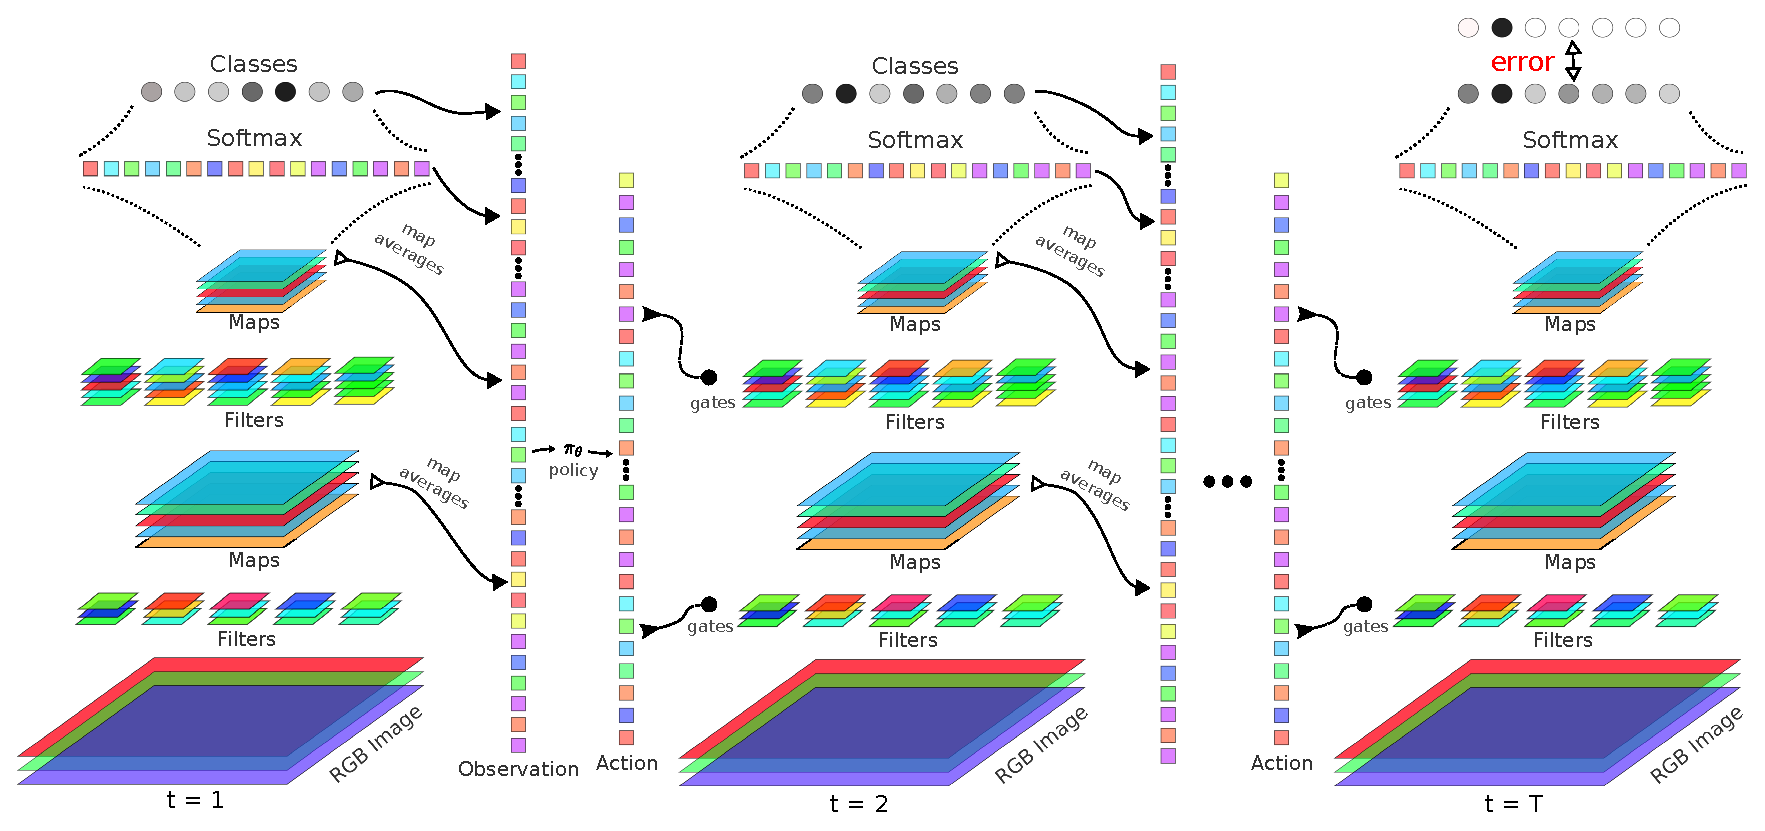
\includegraphics[width=\linewidth]{sead_wide.eps}
%\includegraphics[width=\linewidth]{drawing_2.0.eps}
\caption{{\bf The dasNet Network}. Each image in classified after $T$
  passes through the network.  After each forward propagation through
  the Maxout net, the output classification vector, the output of the
  second to last layer, and the averages of all feature maps, are
  combined into an observation vector that is used by a
  deterministic policy to choose an action that
  changes the weights of all the feature maps for the next pass of the
  same image.  After pass $T$, the output of the Maxout net is finally
used to classify the image.}
\label{fig:model}
\end{figure*}




Once all of the candidate policies have been evaluated, SNES updates
its distribution parameters ($\mu, \Sigma$) according the natural
gradient calculated from the sampled fitness values, $\mathcal{F}$.
As SNES repeatedly updates the distribution over the course of many
generations, the expected fitness of the distribution improves, until
the stopping criterion is met.

%Using minibatches has two advantages: using GPU's it is efficient to
%process several images at once, and it results in a better estimate
%for the fitness of our policy.  

% We argue that dasNet can actively select a subnetwork which
% better suits a given input pattern; this is in sharp contrast to
% approaches like dropout~\cite{Krizhevsky:2012} and
% dropconnect~\cite{wan2013regularization} which are completely
% stochastic and feedforward and do not try to explicitly model the
% network's activity.  

%%%  ???
%We will validate through visual inspection such
%belief in the experimental section.  It is in fact arguable that using
%a large model meets the Occam's razor principle. We rather believe
%that capacity should be very high but usage should be selective and
%minimize some activity criterion.  In other words it is very unlikely
%that we would use all resources in a resource bounded environment.
%%%

\section{Related Work}
%Investigating vision as an interactive and self-adaptive process is
%not novel and has been investigated within psychology from a human
%perspective and in computer vision from an engineering perspective.
Human vision is still the most advanced and flexible perceptual system
known.  Architecturally, visual cortex areas are highly connected,
including direct connections over multiple levels and top-down
connections. \citet{felleman1991distributed} constructed a (now
famous) hierarchy diagram of 32 different visual cortical areas in
macaque visual cortex.  About 40\% of all pairs of areas were
considered connected, and most connected areas were connected 
bidirectionally.  The top-down connections are more numerous than
bottom-up connections, and generally more
diffuse~\cite{douglas1995recurrent}.  They are thought to play 
primarily a modulatory role, while feedforward connections serve as
directed information carriers~\cite{Bullier2004}.

Analysis of response latencies to a newly-presented image lends
credence to the theory that there are two stages of visual processing:
a fast, pre-attentive phase, due to feedforward processing, followed
by an attentional phase, due to the influence of recurrent
processing~\cite{lamme2000distinct}.  After the feedforward pass, we
can recognize and localize simple salient stimuli, which can
``pop-out''~\cite{Itti:2007}, and response times do not increase
regardless of the number of distractors.  However, this effect has
only been conclusively shown for basic features such as color or
orientation; for categorical stimuli or faces, whether there is a
pop-out effect remains
controversial~\cite{francolini1979perceptual,vanrullen2006second}.
Regarding the attentional phase, feedback connections are known to
play important roles, such as in feature
grouping~\cite{gilbert2007brain}, in differentiating a foreground from
its background, (especially when the foreground is not highly
salient~\cite{hupe1998cortical,bullier2001role}), and perceptual
filling in~\cite{lamme2001blindsight}. Work by~\citet{bar2006top}
supports the idea that top-down projections from prefrontal cortex
play an important role in object recognition by quickly extracting
low-level spatial frequency information to provide an initial guess
about potential categories, forming a top-down expectation that biases
recognition.  Recurrent connections seem to rely heavily on
competitive inhibition and other feedback to make object recognition
more robust~\cite{wyatte2012, wyatte2012b}.

In the context of computer vision, RL has been shown to be able to
learn saccades in visual scenes to learn selective
attention~\cite{SchmidhuberHuber:91}, learn feedback to lower levels
\cite{oreilly1996, fukushima2003}, and improve face recognition
\cite{larochelle2010learning,goodrich2012reinforcement,stollenga2011using}.
It has been shown to be effective for object recognition
\cite{oreilly2013}, and has also been combined with traditional
computer vision primitives ~\cite{Whitehead:92}. Iterative processing
of images using recurrency has been successfully used for image reconstruction
\cite{behnke2001learning} and face-localization \cite{behnke2005face}.
All these approaches show that recurrency in processing and an RL perspective can lead to
novel algorithms that improve performance.  However, this research is
often applied to simplified datasets for demonstration purposes due to
computation constraints, and are not aimed at improving the
state-of-the-art.  In contrast, we apply this perspective directly to
the known state-of-the-art neural networks to show that this approach
is now feasible and actually increases performance.

\section{Experiments on CIFAR-10/100}
\label{sec:experiments}

%This is the case of the cats-vs-dogs challenge
%which has recently arisen lot of interest in the
%community~\cite{WelinderEtal2010}.
The experimental evaluation of dasNet focuses on ambiguous
classification cases in the CIFAR-10 and CIFAR-100 data sets where,
due to a high number of common features, two classes are often
mistaken for each other.  These are the most interesting cases for our
approach.  By learning on top of an already trained model, dasNet must
aim at fixing these erroneous predictions without disrupting, or
forgetting, what has been learned.

The CIFAR-10 dataset~\cite{krizhevsky:2009} is composed of $32 \times
32$ color images split into $5 \times 10^4$ training and $10^4$
testing samples, where each image is assigned to one of $10$ classes.
The CIFAR-100 is similarly composed, but contains $100$ classes.
%It is important to consider that often there are only very little
%mistakes in the training set.  Even with such data scarcity we show
%that we are able to improve the state-of-the-art.

%{\em It is now the question of how much capacity is wasted because 
%a more principled model with feedback connections has not been used. 
%[this is for later, but we should ask this question]}

%\emph{Argue why cifar is perfect and we dont need much more.}
%{\bf did not we have a better result on cifar?}

The number of steps, $T$, for the RL was experimentally determined and
fixed at $5$; enough steps to allow dasNet to adapt while being small
enough to be practical.  While it is be possible to iterate until some
condition is met, this could be a serious limitation in real-time
applications where predictable processing latency is critical.  In all
experiments we set $\lambda_{\text{correct}} = 0.005$,
$\lambda_{\text{misclassified}} = 1$ and $\lambda_{\text{L2}} =
0.005$.



\begin{figure}[t]
\begin{minipage}[b]{0.55\linewidth}
\begin{tabular}{l c c}
  \hline
  Method & {\footnotesize CIFAR-10} & {\footnotesize  CIFAR-100} \\
  \hline
  \hline
  Dropconnect~\cite{wan2013regularization}% ({\footnotesize 12 CNNs}) 
& 9.32\% & -\\
  \hline
  Stochastic Pooling~\cite{2013:zeiler_stochpool} & 15.13\% & - \\ 
  Multi-column CNN~\cite{ciresan2012cvpr} & 11.21\% & - \\
  Maxout~\cite{goodfellow2013maxout} & 9.38\% & 38.57\% \\
  Maxout (our model) & 9.61\% & 34.54\% \\
  \bf{dasNet} & \bf{9.22}\%  & \bf{33.78}\% \\ 
  \hline
\end{tabular}
\captionof{table}{Classification results on CIFAR-10 and CIFAR-100
  datasets. The error on the test-set is shown for several methods.
  Note that the result for Dropconnect is the average of 12
  models. Our method improves over the state-of-the-art reference
  implementation to which feedback connections are added.  }
\label{tab:cifar10}
\end{minipage}
\quad
\begin{minipage}[b]{0.4\linewidth}
\centering
\includegraphics[angle=-90,width=\linewidth]{1step2step.eps}
\caption{Two dasNets were trained on CIFAR-100 for different values of $T$.
Then they were allowed to run for [0..9] iterations for each image. 
The performance peeks at the number of steps that the network is trained on, 
after which the performance drops, but does not explode, showing the dynamics are stable.}
\label{fig:1step2step}
\end{minipage}
\hspace{0.5cm}
\end{figure}



%The classes range from `cat' and 'fish' to `truck', `vegetables' and
%`household furniture'.


The Maxout network, $\mathbf{M}$, used in the experiments was trained
with data augmentation following the suggested global contrast
%% who "suggested"?
normalization and ZCA normalization protocol.  The model consists of
three convolutional maxout layers followed by a fully connected maxout
and softmax outputs. Dropout of $0.5$ was used in all layers except the
input layer, and $0.2$ for the input layer.  The population size for
SNES was set to 50.

%\emph{pylearn2} 


%\subsection{Results}
Table~\ref{tab:cifar10} shows the performance of dasNet vs. other
methods, where it achieves a relative improvement of $6\%$ with
respect to the vanilla CNN.  This establishes a new state-of-the-art
result for this challenging dataset.

Figure~\ref{fig:details1} shows the classification of a cat-image from
the test-set.  All output map activations in the final step are shown
at the top. The difference in activations compared to the first step,
i.e., the (de-)emphasis of each map, is shown on the bottom. On the
left are the class probabilities for each time-step. At the first
step, the classification is `dog', and the cat could indeed be mistaken
for a puppy. Note that in the first step, the network has not yet
received any feedback.  In the next step, the probability for `cat' goes up
dramatically, beating 'dog', and subsequently drops a bit in the
following steps.  The network has successfully disambiguated a cat
from a dog. If we investigate the filters, we see that already in the
lower layer emphasis changes significantly. Some filters focus more on
surroundings whilst others de-emphasize the eyes. %Note
%that the activation differences are shown normalized, and do not
%necessarily completely remove activations, instead they seem to
%balance the filters.

In the second layer, almost all output maps are
emphasized. In the third and highest convolutional layer, the most
complex changes to the network. At this level the
positional correspondence is largely lost, and the filters are known
to code for `higher level' features. It is in this layer that changes
are the most influential because they are closest to the final output
layers. 
%%%%%%%%%
%% TINO.  no idea what you're trying to say here
It is hard to analyze the effect of the alterations, but we
can see that the differences are not simple increases or decreases of
the output maps, as we then would expect the final activations and
their corresponding increases to be largely similar. Instead we see
complex emphasis and pattern suppression.
%%%%%%%%%

\paragraph{Dynamics} To investigate the dynamics, a small 2-layer dasNet
network was trained for different values of $T$. Then they were evaluated
by allowing them to run for $[0..9]$ steps.
Figure~\ref{fig:1step2step} shows results of training dasNet on CIFAR-100 for $T=1$ and $T=2$.
The performance goes up from the vanilla CNN, peaks at the $step = T$ as
expected, and reduces but stays stable after that.
So even though the dasNet was trained using only a small number of steps,
the dynamics stay stable when these are evaluated for as many as 10 steps.

To verify whether the dasNet policy is actually making good use of its gates,
their information content is estimated the following way:
The gate values in the last step are taking and used directly for classification.
If the gates are used properly then their activation should contain information that is relevant for classification
and we would expect a

dasNet that was trained with $T=2$ and are used as
features for classification. Then using \emph{only} the final gate-values (so without e.g. the output of the classification layer), 
a classification using 15-nearest neighbour and logistic regression was performed. This
resulted in a performance of \emph{40.70\%} and \emph{45.74\%} correct
respectively, similar to the performance of dasNet, confirming that
they contain significant information and we can conclude that they are purposefully used.

\begin{figure*}[t]
\centering
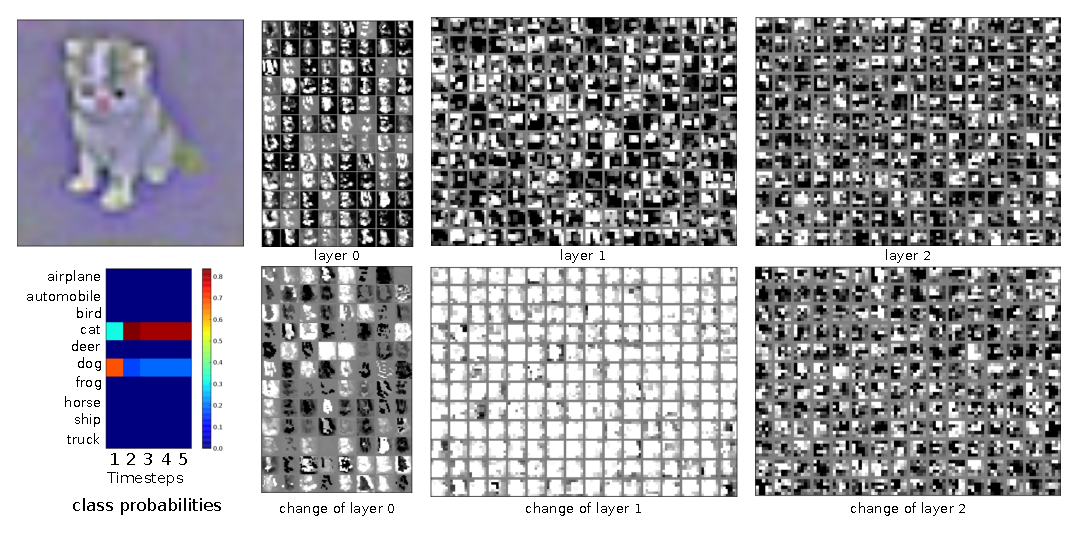
\includegraphics[width=\linewidth]{catdog.eps}
\caption{The classification of a cat by the dasNet is shown. All
  output map activations in the final step are shown on the top. Their
  changes relative to initial activations in the first step
  are shown at the bottom (white = emphasis, black = suppression). The
  changes are normalized to show the effects more
  clearly. The class probabilities over time are shown on the left. The
  network first classifies the image as a dog (wrong) but corrects
  itself by emphasizing its convolutional filters to see it is actually a cat.}
\label{fig:details1}
\end{figure*}


\section{Conclusion}
DasNet is a deep neural network with feedback connections that are
learned by through reinforcement learning to direct selective internal
attention to certain features extracted from images. After a rapid
first shot image classification through a standard stack of
feedforward filters, the feedback can actively alter the importance of
certain filters ``in hindsight'', correcting the initial guess via
additional internal ``thoughts''.
%The filter weights are learned by standard gradient descent. 

DasNet successfully learned to correct image misclassifications
produced by a fully trained feedforward Maxout network. Its active,
selective, internal spotlight of attention enabled state-of-the-art
results.

Future research will also consider more complex actions that spatially
focus on (or alter) parts of observed images.

\section*{Acknowledgments} 
We acknowledge Matthew Luciw, who provided a short literature review, partially included in the Related Work section.

%------------------------------------
%We presented dasNet, a deep neural network which directs selective attention to features
%by actively altering the strength of its convolutional filters. This is achieved by seeing 
%classification as an interactive process, from a reinforcement learning perspective.


%The experiments show that dasNet was able to disambiguate and correct classifications of images that a fully trained Maxout network failed on.
%It thus seems that viewing classification as an interactive process that allows for selective attention is fruitful, and can produce state-of-the-art results.

%The specific actions and observations that were selected in this research
%still seem relatively simple. More complex actions that alter the image itself
%or spatially focus on parts of the image will be explored in the future.


%------------------------------------

%The most appealing property of the proposed approach is not given by
%the classification results but by its ability to learn how to
%disambiguate.  It is interesting to see that the network from a
%dynamical perspective; the network seems to find a stable state, but
%it also wants to push away from misclassifications. 


%To do this, given a prediction, the system can change its sensitivities such that the
%system more strongly tests this classification and is `pushed' away
%from the current state if that is not the case.  From visual
%inspection we can see such interesting correcting behaviours,
%providing evidence for our initial claim.  Further research is needed
%to understand the dynamics deeper.

%In Figure~\ref{fig:details2} another example from the CIFAR-10 dataset
%is shown to further demonstrate the capability of a dasNet to
%disambiguate between hard to classify patterns. It is interesting to
%see that even if after a single iteration the system correctly
%predicts the airplane, it is only after the fourth step that it finds
%a stable classification.  The network seems to actively balance the
%hypothesis until it is attracted to a stable answer.



%\section{Conclusions}
%\label{sec:conclusions}

%Through visual inspection and analysis of the experimental results
%we can confirm that even perfectly trained models can be improved to 
%an even better state-of-the-art.

%This work shows that perhaps adding capacity is not always the best way
%to go as smaller and smarter models could be learned, perhaps 
%jointly merging the RL into the deep learning system from the beginning.

%\section{Acknowledgements}



% Acknowledgements should only appear in the accepted version. 
%\section*{Acknowledgments} 
%Eventually

% In the unusual situation where you want a paper to appear in the
% references without citing it in the main text, use \nocite
% \nocite{langley00}

{
\small
\bibliography{biblio,bib}
\bibliographystyle{unsrtnat}
}

\end{document} 


% This document was modified from the file originally made available by
% Pat Langley and Andrea Danyluk for ICML-2K. This version was
% created by Lise Getoor and Tobias Scheffer, it was slightly modified  
% from the 2010 version by Thorsten Joachims & Johannes Fuernkranz, 
% slightly modified from the 2009 version by Kiri Wagstaff and 
% Sam Roweis's 2008 version, which is slightly modified from 
% Prasad Tadepalli's 2007 version which is a lightly 
% changed version of the previous year's version by Andrew Moore, 
% which was in turn edited from those of Kristian Kersting and 
% Codrina Lauth. Alex Smola contributed to the algorithmic style files.  


